\documentclass{beamer}
\usepackage[utf8x]{inputenc} % Texte d'entrée encodé au format UTF-8
\usepackage[T1]{fontenc} % Texte de sortie encodé au format Latin-1
\usepackage[english]{babel} % If you write in French
\usepackage{array}

\usetheme{Singapore}

\title{Wanna TEMPEST your computer?}
\author{Florian Barbarin, Maxime Gagliardini and Guillaume Squillaci}
\institute{TLS-SEC}
\date{\today}

\AtBeginSection[]
{
  \begin{frame}
  \frametitle{Table of contents}
  \tableofcontents[currentsection,currentsubsection]
  \end{frame} 
}

\begin{document}

\begin{frame}
\titlepage

\begin{table}
\centering
\begin{tabular}{>{\centering\arraybackslash}m{.4\textwidth} >{\centering\arraybackslash}m{.4\textwidth}}

\centering 
\includegraphics[scale=.07]{images/tlssec.png} & 
\centering 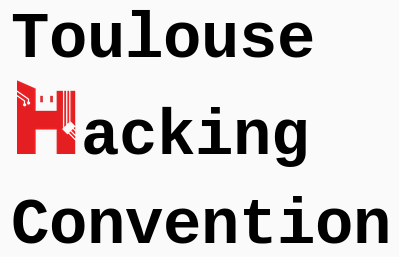
\includegraphics[scale=.3]{images/thc.png}
\end{tabular}
\end{table}
\end{frame}

\section{Introduction}

	\begin{frame}
\frametitle{"Projet long" background}
\begin{block}{THC 2018 Challenge}
\begin{itemize}
\item Prepare tutorial challenge
\item Work based on \textit{GSMem: Data Exfiltration from Air-Gapped 
Computers over GSM Frequencies} (24th USENIX Security Symposium)
\item "Challenge" : data exfiltration form an air-gapped computer
\item "Tutorial" : guide the challenger step-by-step
\item Idea : follow how we succeed to reproduce a part of the paper
\end{itemize}
\end{block}
\end{frame}

\begin{frame}
\frametitle{Electromagnetic emanations}
\begin{block}{Emanations}
\begin{itemize}
\item Each electronic device has emanations
\item Could be electronical, acoustical, mecanical or electromagnetical
\item We focused on electromagnetic emanations
\end{itemize}
\end{block}

\begin{block}{TEMPEST}
\begin{itemize}
\item Name given by NSA for standards protecting against electromagnetic emanations
\item Context : EMSEC, surbpart of COMSEC
\end{itemize}
\end{block}
\end{frame}


\begin{frame}
\frametitle{Air-gapped networks}
\centering 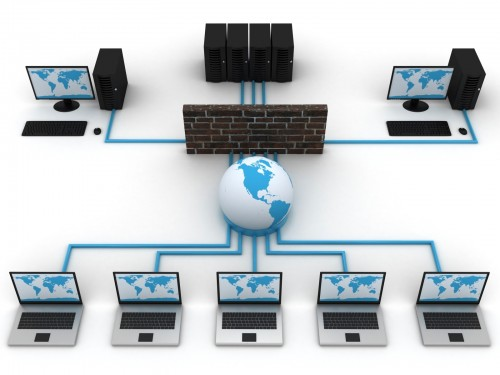
\includegraphics[scale=.5]{images/network.jpg}
\end{frame}

\begin{frame}
\frametitle{Air-gapped networks}
\centering 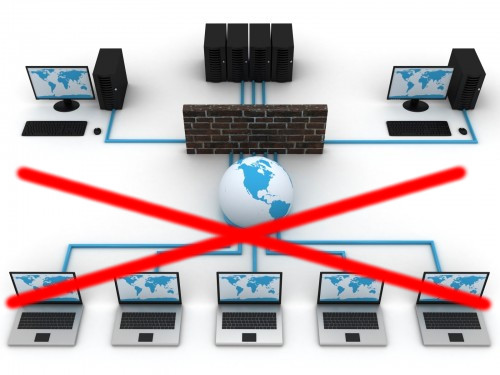
\includegraphics[scale=.5]{images/network2.jpg}
\end{frame}


\begin{frame}
\frametitle{Data exfiltration}
\begin{block}{Devices}
\begin{itemize}
\item 1 air-gapped computer (attacked computer)
\item 1 standard computer (attacker's computer)
\end{itemize}
\end{block}

\begin{block}{Tools}
\begin{itemize}
\item Spectrum analyzer
\item Software-defined radio : USRP/RTL-SDR
\item Antennas
\item Softwares : URH/GNURadio
\end{itemize}
\end{block}

\begin{block}{Goal}
Transfer a password from the air-gapped computer to the attacker's computer creating a covert channel.
\end{block}

%\begin{center}
%
\includegraphics[scale=.37]{images/com.pdf}
%\end{center}
\end{frame}

\section{Transmitter}

	\begin{frame}
\frametitle{Transmission without specific component}
\begin{block}{Our target (remind)}
Use electromagnetic emanations to create a covert channel and exfiltrate data
\end{block}
\begin{alertblock}{Problems}
\begin{itemize}
\item Computer's electromagnetic emanations $\rightarrow$ low amplitude
\item Amplitude increase $\Rightarrow$ circuit tension increase
\end{itemize}
\end{alertblock}
\end{frame}

\begin{frame}
\frametitle{Problem bypass : Multi-channel memory architectures}

\begin{columns}[c] % align columns
\begin{column}{.28\textwidth}
\centering 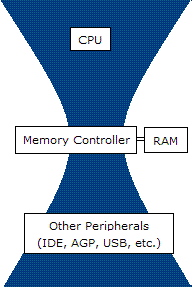
\includegraphics[scale=.3]{images/goulot.png}
\end{column}%
\hfill%
\begin{column}{.68\textwidth}
\begin{block}{Memory access}
\begin{itemize}
\item Memory controller $\rightarrow$ bottleneck
\item Intel/AMD $\rightarrow$ Multi-channel memory architectures
\item Increase data bus size :
\begin{itemize}
\item Double channel $\Rightarrow$ 128 bits
\item Triple channel $\Rightarrow$ 192 bits
\item Quadruple channel $\Rightarrow$ 256 bits
\end{itemize}
\end{itemize}
\end{block}
\end{column}%
\end{columns}

\end{frame}

\begin{frame}
\frametitle{Problem bypass : Multi-channel memory architectures}

\begin{columns}[c] % align columns
\begin{column}{.33\textwidth}
\centering 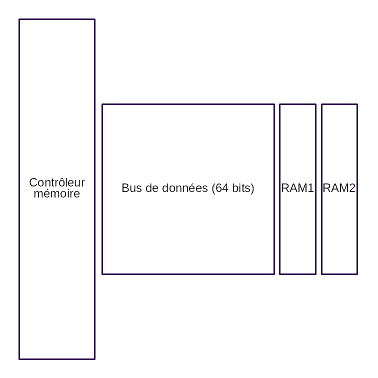
\includegraphics[scale=.4]{images/mono-canal.png}
\end{column}%
%\hfill%
\begin{column}{.01\textwidth}
$\longrightarrow$
\end{column}
\begin{column}{.28\textwidth}
\centering 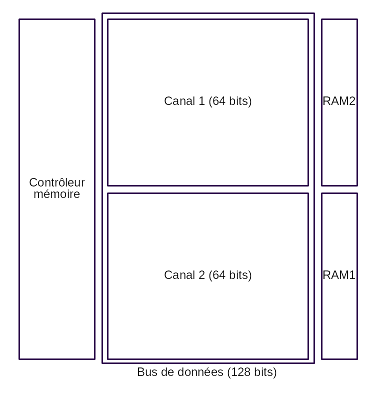
\includegraphics[scale=.4]{images/multi-canal.png}
\end{column}%
\end{columns}

\begin{block}{Consequence using Multi-channel memory}
\begin{itemize}
\item More electrons in movement at the same time
\item Significant electromagnetic emanations created
\item $\Rightarrow$ Emanations could be used to create covert channel
\end{itemize}
\end{block}

\end{frame}

\begin{frame}
\frametitle{Problem bypass : Multi-channel memory architectures}

\begin{columns}[c] % align columns
\begin{column}{.28\textwidth}
\centering 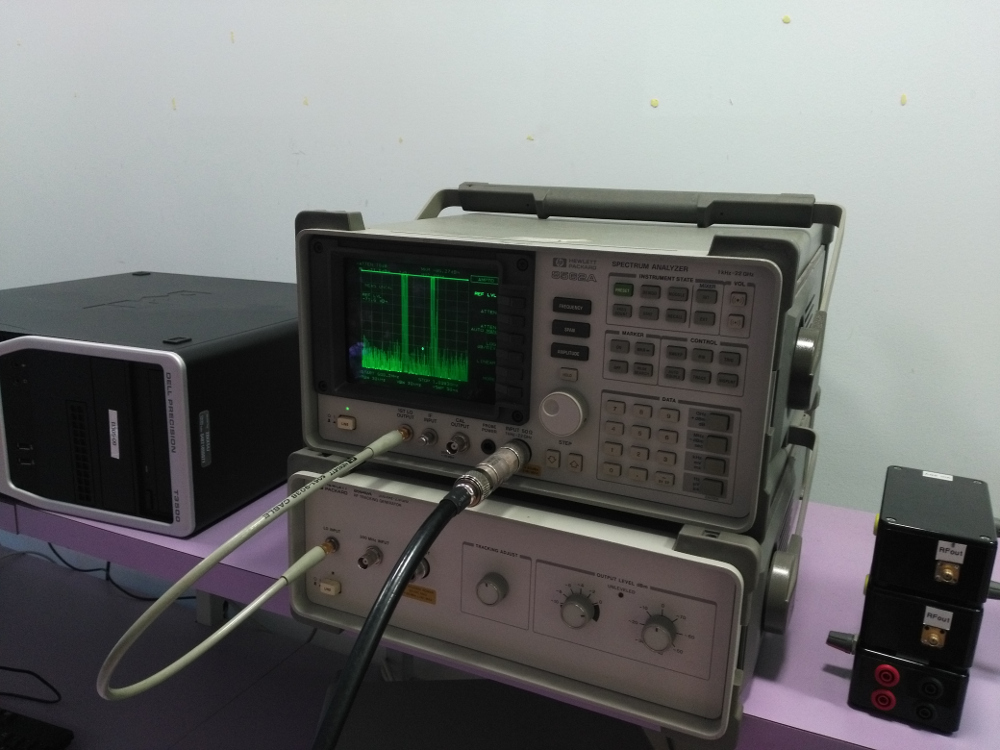
\includegraphics[scale=.13]{images/spectrum.jpg}
\end{column}%
\hfill%
\begin{column}{.5\textwidth}
\begin{block}{Application}
\begin{itemize}
\item Be sure to bypass CPU optimizations
\item Use of \texttt{MOVNTDQ} instruction on \texttt{xmm} registers
\item Emanations highlight :
\begin{itemize}
\item Find emission frequency : spectrum analyzer
\item Watch signal : USRP/RTL-SDR + URH
\end{itemize}
\end{itemize}
\end{block}
\end{column}%
\end{columns}

\end{frame}



\begin{frame}
\frametitle{Problem bypass : Multi-channel memory architectures}

\centering 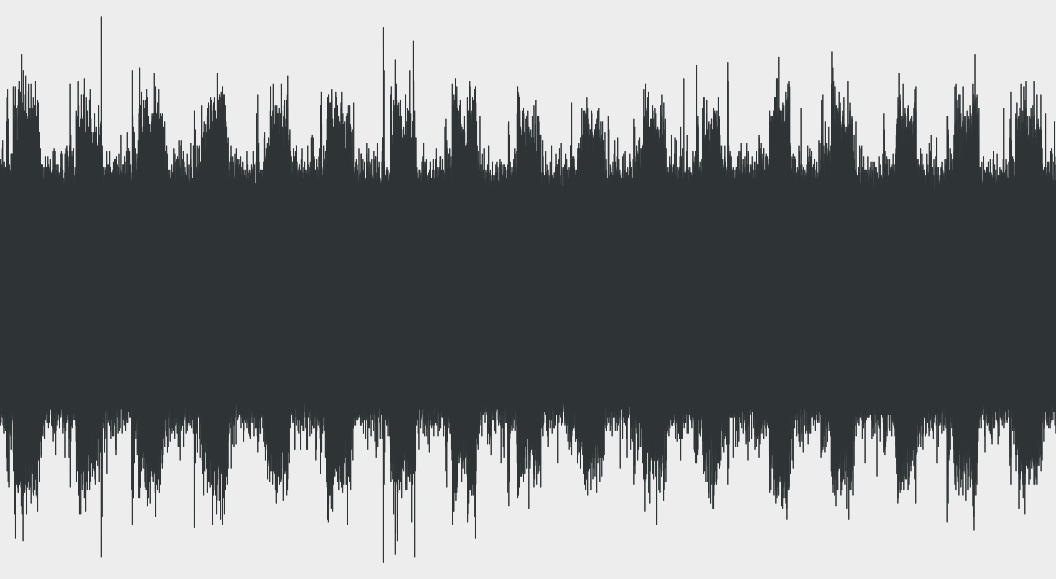
\includegraphics[scale=.2]{images/signal.png}

\begin{block}{Modulation}
\begin{itemize}
\item Modulation = information coding process
\item Binary Amplitude-Shift Keying (B-ASK) modulation :
\begin{itemize}
\item bit 0 $\leftrightarrow$ normal emission level
\item bit 1 $\leftrightarrow$ average emission level when multi-channel memory is used
\end{itemize}
\end{itemize}
\end{block}

\end{frame}

\section{Receiver}

	
\begin{frame}
	\frametitle{Demodulation}
	\centering 
\includegraphics[scale=.13]{images/gnuradio_logo.png}

	\begin{columns}[c] % align columns
		\begin{column}{.28\textwidth}
			\begin{block}{GNUradio}
				\begin{itemize}
					\item Free and Open-source Software
					\item Software Radio
					\item Signal Processing
				\end{itemize}
			\end{block}
		\end{column}%
		\hfill%
		\begin{column}{.5\textwidth}
			\begin{block}{Configuration}
				\begin{itemize}
					\item Sample Rate 
					\item Frequency
					\item Period
					\item Gain
				\end{itemize}
			\end{block}
		\end{column}%
	\end{columns}
\end{frame}

\begin{frame}
	\frametitle{Raw Signal}
	\centering 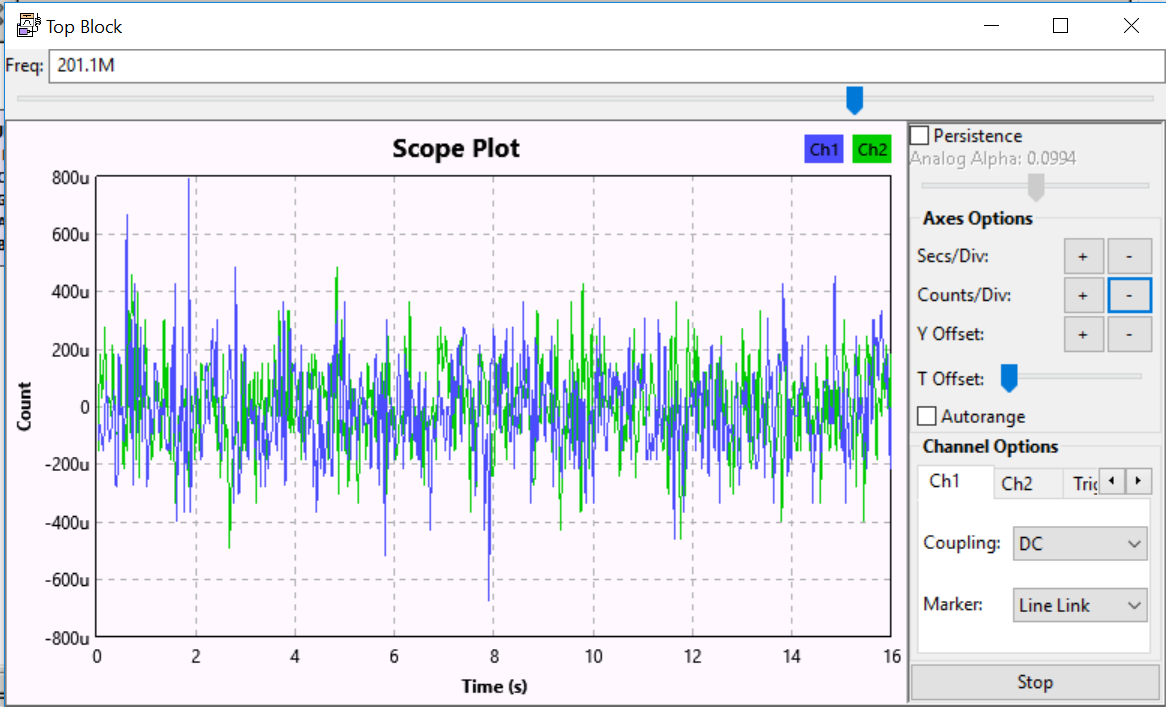
\includegraphics[scale=.2]{images/raw_sig.png}
	\begin{block}{Source Output}
		\begin{itemize}
			\item Complex Signal:
			\begin{itemize}
				\item In-phase 
				\item Quadrature
			\end{itemize}
			\[s(t)=i(t)+jq(t)=r(t).e^j\phi(t) \]
		\end{itemize}
	\end{block}
\end{frame}

\begin{frame}
	\frametitle{Instantaneous Power}
	\centering 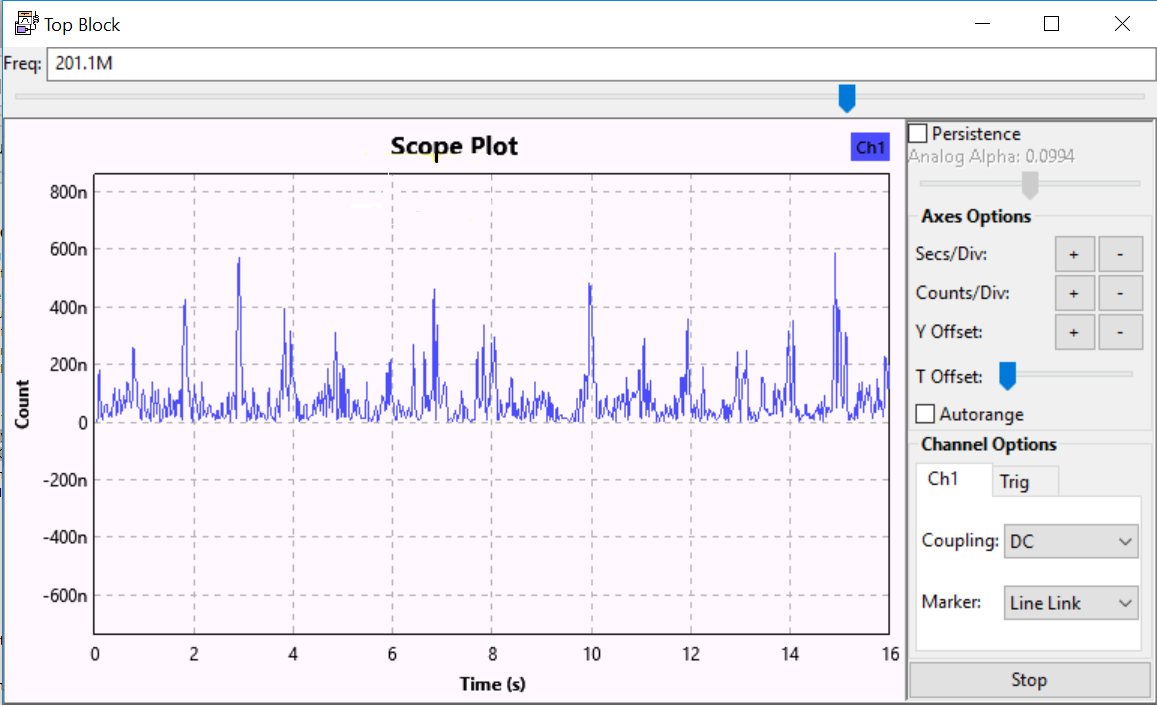
\includegraphics[scale=.2]{images/apres_mag2.png}
	\begin{block}{Float Signal}
		\begin{itemize}
			\item Amplitude
			\item Magnitude
			\[P(t)=|r(t)|²\]
		\end{itemize}
	\end{block}
\end{frame}

\begin{frame}
	\frametitle{Sliding Average}
	\centering 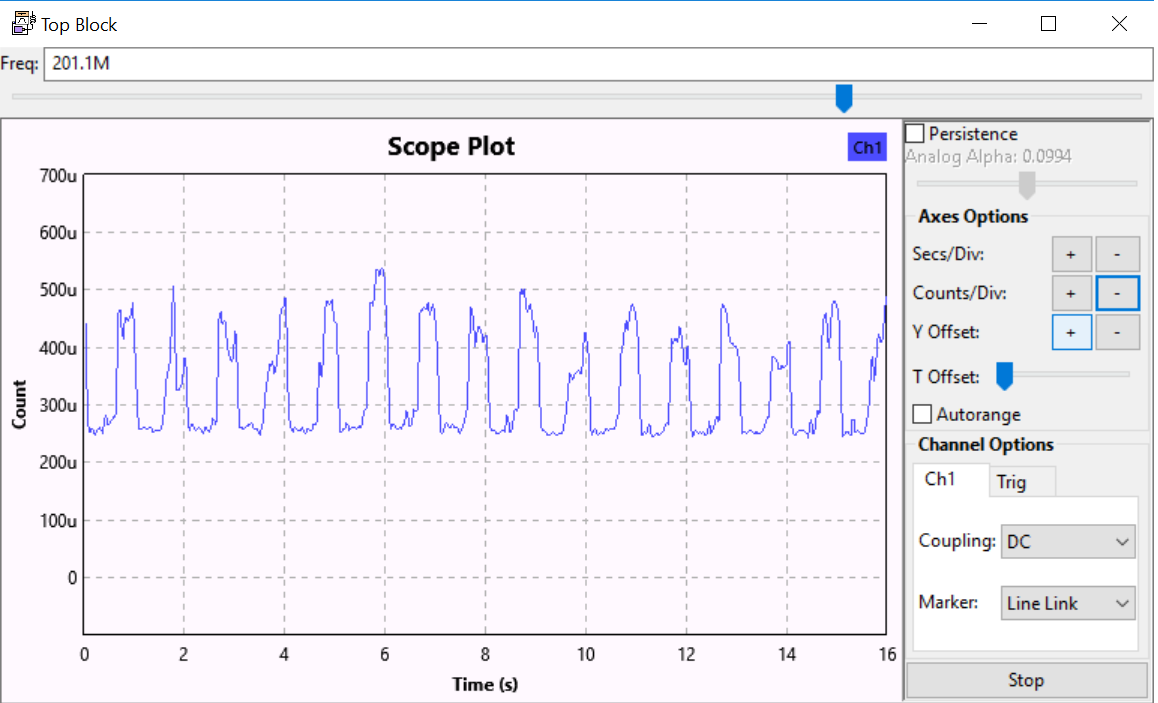
\includegraphics[scale=.2]{images/apres_average.png}
	\begin{block}{Float Signal}
		\begin{itemize}
			\item Number of samples
			\item Treshold
		\end{itemize}
	\end{block}
\end{frame}

\begin{frame}
	\frametitle{Signal Before Decision}
	\centering 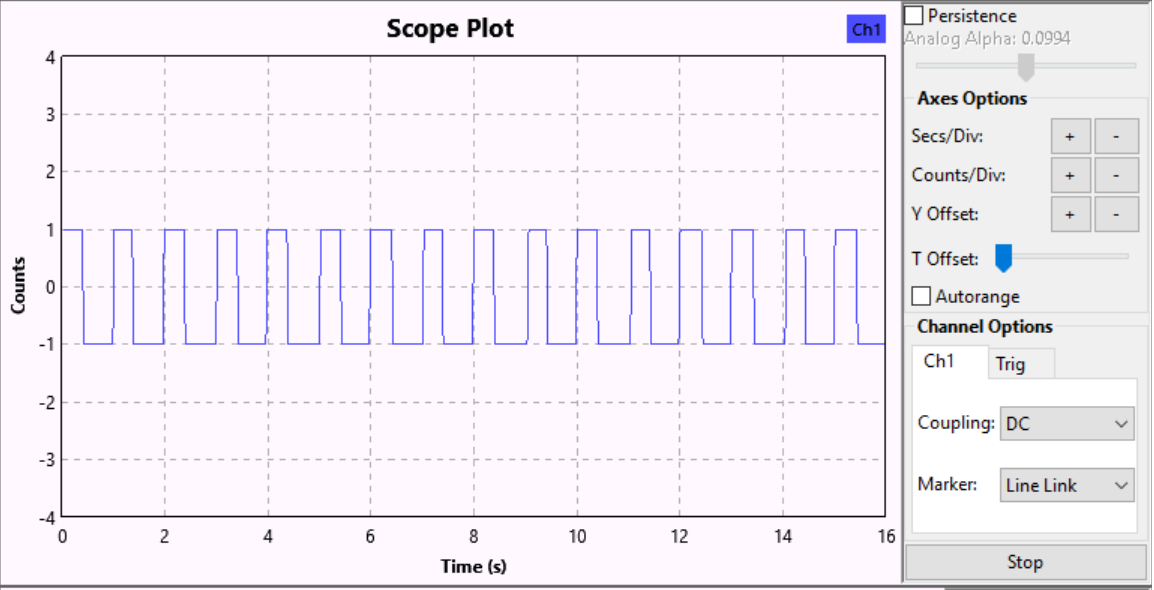
\includegraphics[scale=.2]{images/apres_add_const.png}
	\begin{block}{Square Wave}
		\begin{itemize}
			\item Clock period
			\item Output Byte
			\item Byte Processing
		\end{itemize}
	\end{block}
\end{frame}

\begin{frame}
	\frametitle{Conclusion}
	\begin{block}{Problem}
		\begin{itemize}
			\item Noise
			\item Synchronization
			\item Transmitter
			\item BER
		\end{itemize}
	\end{block}
\end{frame}

	
\section{Data exfiltration}

	\begin{frame}
\frametitle{The Malware}
\begin{block}{Idea}
\begin{itemize}
\item Same skeleton than the Transmission section
\item 1bit/s to reduce error rate
\end{itemize}
\end{block}
\begin{block}{What is transmitted ?}
\begin{itemize}
\item The message : a file in argument
\item End of File : 00001010
\item A pattern to localize the message : 11111111
\item All of this in an infinite loop
\end{itemize}
\end{block}
\end{frame}

\begin{frame}
\frametitle{Reception}
\begin{block}{In GNU Radio}
\begin{itemize}
\item Start the malware before the acquisition to avoid a bug in the first bit transmitted
\item Wait around 2 minutes
\end{itemize}
\end{block}
\begin{block}{Conversion of the GRC file into our flag}
\begin{itemize}
\item Localize a first pattern
\item Extract bytes from this pattern until the next one
\item Convert extracted bytes into ASCII and print it
\end{itemize}
\end{block}
\end{frame}

\begin{frame}
\frametitle{Reception}
\centering 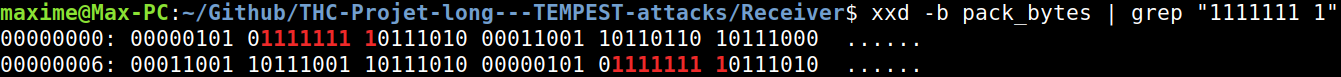
\includegraphics[scale=0.22]{images/xxd1.png}\\
\null
\centering 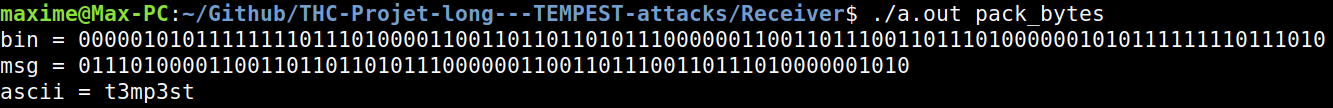
\includegraphics[scale=0.22]{images/xxd2.png}
\end{frame}

\begin{frame}
\frametitle{Reception}
\centering 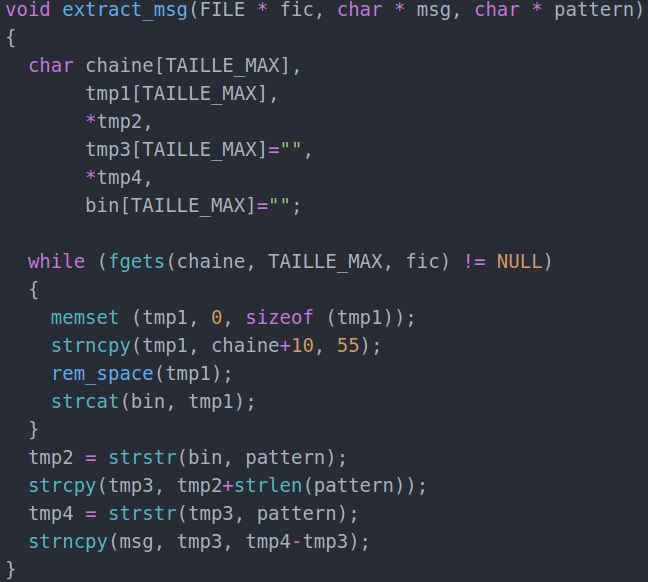
\includegraphics[scale=0.38]{images/extract_message.png}
\end{frame}
	
\section{Conclusion}

	\begin{frame}
\frametitle{Conclusion}
\begin{block}{Researchers work}
\begin{itemize}
\item Better equipment
\item Signal processing optimization
\item Reception up to 30m
\end{itemize}
\end{block}
\begin{block}{Limits}
\begin{itemize}
\item Very limited flow rate to prevent error (error detection ?)
\item Can be improve with a frequency modulation (USBee attack)
\end{itemize}
\end{block}
\begin{block}{Countermeasures}
\begin{itemize}
\item Faraday cage
\item Zonal approach
\item Antivirus
\end{itemize}
\end{block}
\end{frame}


\end{document}